\usetikzlibrary{arrows}
\usetikzlibrary{fit}

\tikzset{
	pics/conv/.style n args={5}{
		code = {
			\draw[draw=black] (#1, #2) rectangle ++ (1, 3) node[rotate=90, pos=0.5] {\large $#3 \times #4 \times #3$};
			\node[below] at (#1+0.5, #2+3.1) {\large #5};
		}
	},
	pics/text/.style n args={5}{
		code = {
			\draw[draw=black] (#1, #2) rectangle ++ (1, 3) node[rotate=#4, pos=0.5] {\huge #3};
			\node[below] at (#1+0.5, #2+3.1) {\large #5};
		}
	}
}

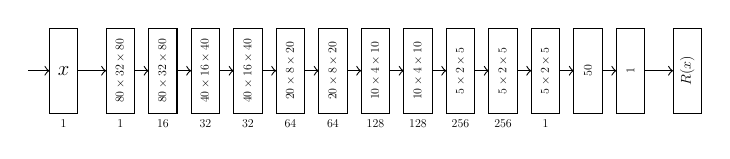
\begin{tikzpicture}[scale=0.36, line/.style={>=latex}, every node/.style={scale=0.36}, y=-1cm] 
	% --- critic ---
	%\pic{text={0}		{15}	{$x\vphantom{xyt}$}	{0}	{1}};
	%\pic{text={1}		{15}	{$y\vphantom{xyt}$}	{0}	{1}};
	\pic{text={2}		{15}	{$x\vphantom{xyt}$}	{0}	{1}};

	\pic{conv={4}		{15}	{80}	{32}	{1}};
	\pic{conv={5.5}		{15}	{80}	{32}	{16}};
	\pic{conv={7.0}		{15}	{40}	{16}	{32}};
	\pic{conv={8.5}		{15}	{40}	{16}	{32}};
	\pic{conv={10.0}	{15}	{20}	{8}	{64}};
	\pic{conv={11.5}	{15}	{20}	{8}	{64}};
	\pic{conv={13.0}	{15}	{10}	{4}	{128}};
	\pic{conv={14.5}	{15}	{10}	{4}	{128}};
	\pic{conv={16}		{15}	{5}	{2}	{256}};
	\pic{conv={17.5}	{15}	{5}	{2}	{256}};
	
	\pic{conv={19}		{15}	{5}	{2}	{1}};
	
	\pic{text={20.5}	{15}	{\large $50$}	{90} {}};
	\pic{text={22}		{15}	{\large $1$}	{90} {}};
	
	\pic{text={24}		{15}	{\Large $R(x)\vphantom{xyt}$}	{90}	{}};

	\draw[->] (1.25, 16.5) -- (2, 16.5);
	\draw[->] (3, 16.5) -- (4, 16.5);

	\draw[->] (5, 16.5) -- (5.5, 16.5);
	\draw[->] (6.5, 16.5) -- (7, 16.5);
	\draw[->] (8, 16.5) -- (8.5, 16.5);
	\draw[->] (9.5, 16.5) -- (10, 16.5);
	\draw[->] (11, 16.5) -- (11.5, 16.5);
	\draw[->] (12.5, 16.5) -- (13, 16.5);
	\draw[->] (14, 16.5) -- (14.5, 16.5);
	\draw[->] (15.5, 16.5) -- (16, 16.5);
	\draw[->] (17, 16.5) -- (17.5, 16.5);
	\draw[->] (18.5, 16.5) -- (19, 16.5);
	\draw[->] (20, 16.5) -- (20.5, 16.5);
	\draw[->] (21.5, 16.5) -- (22, 16.5);
	\draw[->] (23, 16.5) -- (24, 16.5);


\end{tikzpicture}
